\section{Mittelfristige Projekte}
\label{sec:Mittelfristige Projekte}

Nach der Einarbeitungszeit und dem Kennenlernen der Hard- und Software wurde mir nach ca. 2 Monaten mein erstes eigenes Projekt überlassen. In diesem ging es um die ganzheitliche Planung, Organisation und Umsetzung von innerbetrieblichen Schulungen. Bei diesen Schulungen handelte es sich um SQL-, Azure-, SAP- und weitere spezielle Mitarbeiter-Schulungen. Diese Schulungen wurden regelmäßig von der DKB-Management-School geplant und finanziert. Dabei wurde in der Regel folgende Komponenten für eine Schulung benötigt:
\begin{itemize}
	\item Schulungs-Laptop
	\item Switches
	\item LAN-Kabel
	\item Netzteile
	\item Steckdosen
	\item Mäuse
\end{itemize}
\noindent
Mein Aufgabenbereich erstreckte sich von der Annahme der Tickets für Schulungen, der Beschaffung der korrekten Hardware, dem Buchen der Schulungs-Hardware, dem Verschicken der richtigen Hardware bis zur Organisation des Aufbaus beim Kunden. Im weiteren Verlauf versuchte ich den Prozess des Buchens von Hardware zu optimieren, indem ich eine eigene Buchungsseite programmierte, welche mit einer Datenbank kommunizierte die auf einem Server bei uns im Büro stand. Die Seite sollte schlicht und übersichtlich gehalten werden und wurde in Python geschrieben. Um abrufen zu können welche Laptops gebucht wurden, habe ich im weiteren Verlauf ein kleines Programm mit Benutzeroberfläche geschrieben, welches mit der Datenbank kommunizieren und die jeweiligen Einträge ausgeben und verändern konnte. So war es deutlich einfacher einen Überblick zu bekommen, welche Rechner gebucht und welche verfügbar waren. Jeder Buchung wurde das entsprechende Ticket zugeordnet und es konnte ein Blatt ausgedruckt werden, welches die genauen Hardwareanforderungen für die jeweilige Schulung enthielt. Nach einer Buchung wurde automatisch einen E-Mail mit dem Protokoll im Anhang an meine E-Mail geschickt, sodass ich sofort einen guten Überblick über die anstehende Schulung hatte. Im Prozess davor musste jeder Laptop in einer anderen Datenbank gesucht und gebucht werden. Danach musste das Übergabeprotokoll händisch ausgefüllt und ausgedruckt werden. Zudem musste irgendwo festgehalten werden, welche Laptops verschickt wurden. Der gesamte Prozess war recht unübersichtlich und beinhaltete mehrere Schritte. Durch die Ticketseite konnte der Prozess des Buchens und der Vorbereitung einer Schulung deutlich schneller durchgeführt werden. Außerdem optimierte ich die Erstellung des entsprechenden Übergabeprotokolls, welches die Korrektheit der Lieferung bestätigen sollte. Dazu implementierte ich in dem Datenbank-Programm die Funktion direkt per Knopfruck ein Übergabeprotokoll für die gebuchte Hardware zu erstellen. Während der ganzen Zeit stand mir ein Kollege zur Seite, welcher sich besonders gut mit Netzwerken und Datenbanken auskannte, sodass ich immer einen Ansprechpartner hatte. Im Bereich Datenbanken konnte ich zudem auf die Grundkenntnisse aus dem Modul Datenbanken zurückgreifen. Besonders das Wissen um die dritte Normalform und das Vermeiden von Redundanzen machte sich hier bezahlt. In Projekten in den Modulen Softwaretechnik und Datenbanken konnte ich Erfahrung in der Python-Programmierung sammeln, welche mir die Umsetzung der Projekte im Rahmen der Arbeit bei der DKB ermöglichte. Nach der erfolgreichen Buchung und Vorbereitung einer Schulung, musste ich den Aufbau organisieren. Dazu wurde eine externe Firma beauftragt, bei der es sich um die Schindler AG handelte, welche ich vor jeder Schulung mit einer Woche Vorlauf telefonisch kontaktierte und einen Aufbau koordinierte. Wenn Probleme mit den Terminen bei Schindler auftraten, dann bin ich persönlich zum jeweiligen Standort der Schulung gefahren und habe die Hardware entsprechend aufgebaut. Dabei mussten alle Laptops verkabelt, hochgefahren und betriebsbereit konfiguriert werden. Abschließend wurde ein Netzwerk aufgebaut, welches eine Kommunikation mit dem Netz der DKB gewährleistete. Dazu wurde ein oder mehrere Switches mit dem Netzwerk verbunden, indem die im Büro befindlichen Steckdosen für das Hauseigene Netzwerk verwendet wurden. Danach wurden die Laptops mit dem Switch verbunden, sodass alle auf das Netzwerk zugreifen konnten. Bei dem Netzwerk der DKB handelte es sich um zwei voneinander gekoppelte Netzwerke, welche in ein Bank- und ein Servicenetz gegliedert wurden. In einem großen Vorhaben unter dem Projektnamen Netz 4.0 sollten diese Netze miteinander fusioniert werden, was jedoch nach drei Anläufen bis heute nicht gelang. So musste meist ein Netzwerk für das Bank-Netz hergestellt werden, sodass die Schulungsmitglieder zugriff auf die SQL- oder Bank-Server hatten. Fehlerhafte Hardware musste entsprechend ausgetauscht oder repariert werden. Bei der Zusammensetzung der Hardware musste darauf geachtet werden, dass von bestimmten anfälligen Hadrwarekomponenten mehr als gefordert verschickt wurden, sodass kaputte Komponenten kompensiert werden konnten. Mit der Zeit bekam ich ein Gefühl dafür, welche Hardware oft kaputt geht. So waren es in der Regel Kabel und Netzteile, welche in der Zeit öfter kaputt gingen. Ab und zu mussten auch Switches ausgetauscht werden, was jedoch kein Problem darstellte, da ich meist zwei Switches mehr als gefordert versendete. 
\\
Es kam vor, dass Kunden besondere Anforderungen an eine Schulung hatten, welche entsprechend von mir besorgt und bereitgestellt werden mussten. Dabei ging es in der Regel mehr um Softwareanforderungen, als um Hardware. Da die Laptops entsprechend gehärtet wurden, sodass keine externen Programme einfach aufgespielt werden konnten, stellte dies oft ein Problem dar. Dieses konnte nur gelöst werden, indem ein komplett unabhängiges Betriebssystem installiert wurde, welches ein Aufspielen externer Software erlaubte. Nach Beendigung der Schulungen musste dieser Prozess wieder rückgängig gemacht werden und das alte Betriebssystem aufgespielt werden. Desweiteren musste ich entsprechende Teilnehmer-Accounts auf den Laptops einrichten, welche eine zeitliche Begrenzung hatten und jedem Mitarbeiter entsprechend zugeordnet werden konnten.
In diesem Projekt lernte ich vor allem die Kommunikation und die Zusammenarbeit mit verschiedensten Bereichen und Kollegen kennen und konnte meine Fähigkeiten im Bereich der Programmierung von Datenbanken und Web-Anwendungen verbessern und trainieren.Weiterhin wurde mein Organisationsfähigkeit und das Verständnis der Umsetzung von Hard- und Softwareanforderungen geschult. 

\subsection{Die Buchungsseite für Schulungshardware}
\label{Die Buchungsseite für Schulungshardware}

\begin{figure}[H] 
  \centering
     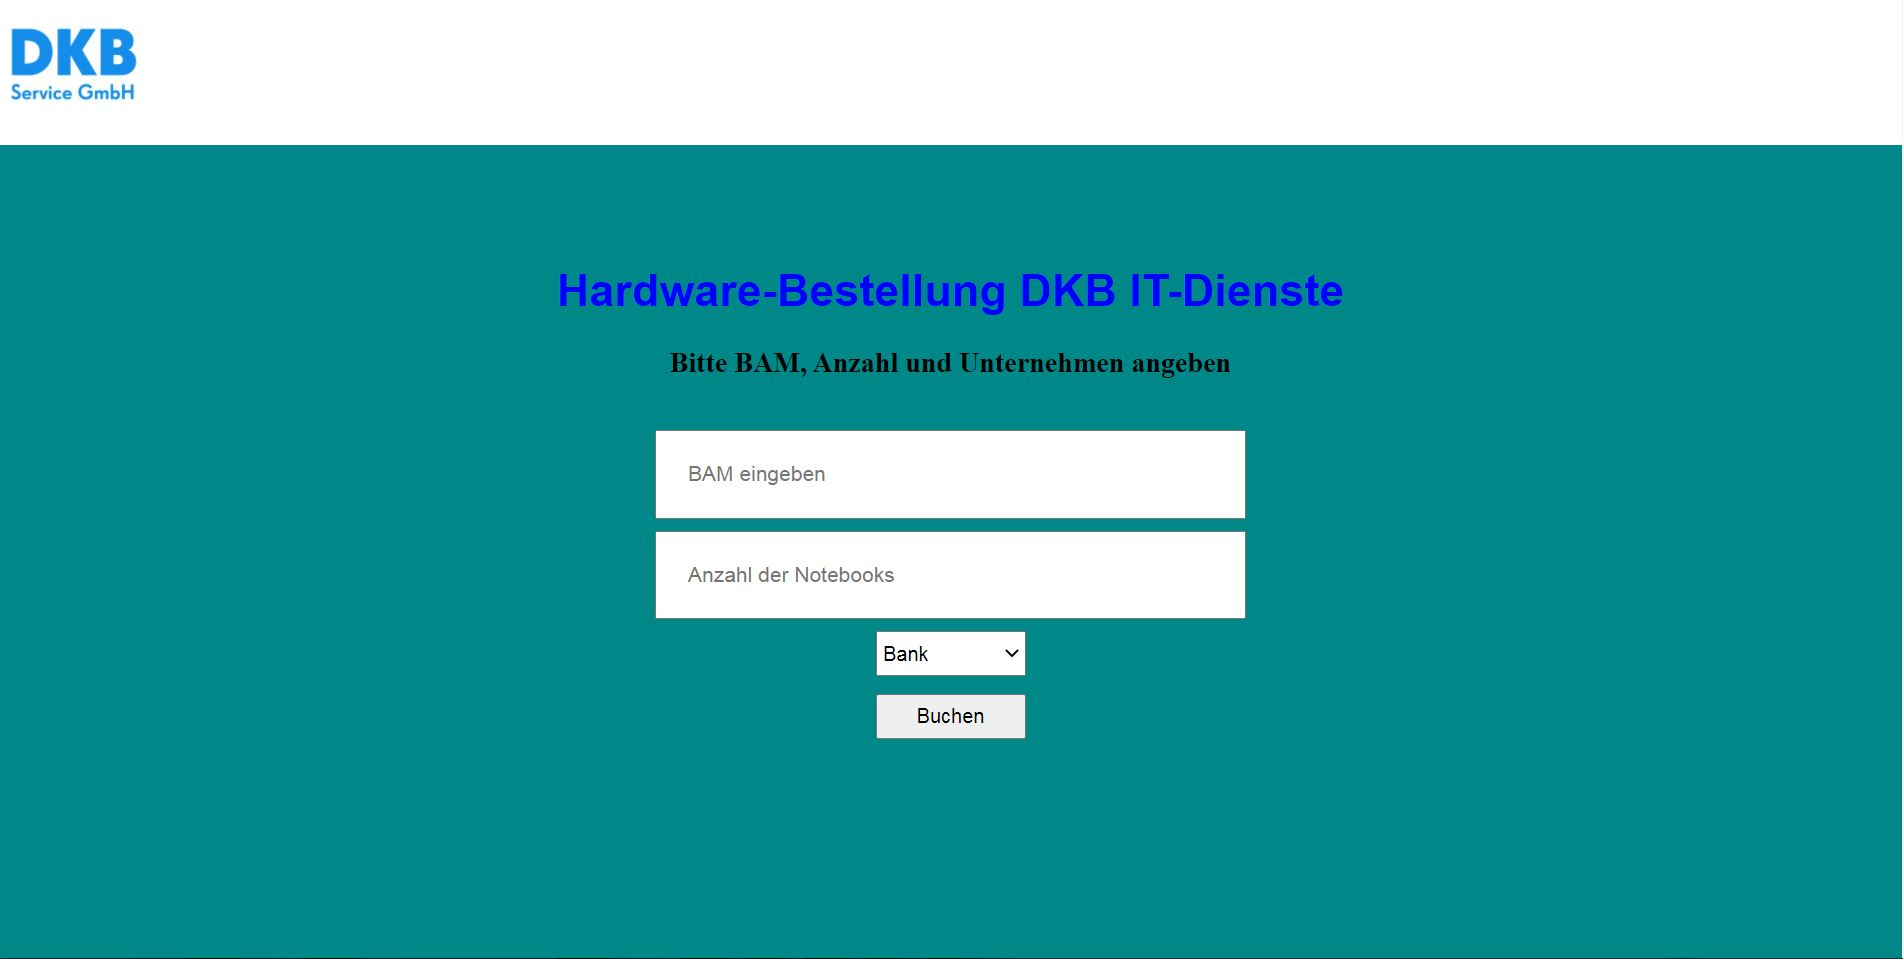
\includegraphics[width=1\textwidth]{ticketseite.jpg}
  \caption{Ticket-Seite}
  \label{fig:Bild1}
\end{figure}

\noindent
Wie auf Abbildung 1 zu erkennen ist, wurde die Seite sehr schlicht gehalten. Sie besteht aus drei HTML-Dateien, welche mit CSS \textit{gestyled} wurden. Die drei HTML-Dateien sind:

\begin{itemize}
	\item error.html
	\item index.html
	\item success.html
\end{itemize}

\noindent
Die index.html stellt die Hauptseite dar, welche beim Start angzeigt wird. Sollte einen Buchung erfolgreich sein, dann wird die nächste seite success.html und bei einem Fehler entsprechend error.html von dem Server aufgerufen. Die Datei app.py beinhaltet den Webserver und die Rendertemplate. Weiterhin wurde hier die Funktionalität des Sendens einer E-Mail bei einer Buchung aufgerufen. Es wurden folgende Bibliotheken verwendet:
\begin{itemize}
	\item flask
	\item request
	\item webbrowser
\end{itemize}

\noindent
Als Datenbank wurde eine einfache DB-Datei verwendet, welche entsprechend durch das Programm mit GUI verändert werden kann. Das Programm zum Bearbeiten der Datenbank besteht dabei aus einem Front- und einem Backend. Im Backend wurden die Funktionalitäten definiert während im Frontend die GUI gezeichnet und die Schnittstelle zwischen Backend und Datenbank geknüpft wird. In der Datenbank wurden die Latops mit Seriennummer, Name, Hersteller und Verfügbarkeit eingepflegt. Pool bedeutete dabei, dass die Laputops verfügbar waren. Über das Programm konnten der Datenbank weitere Laptops hinzugefügt oder alte bearbeitet werden.
\begin{figure}[H] 
  \centering
     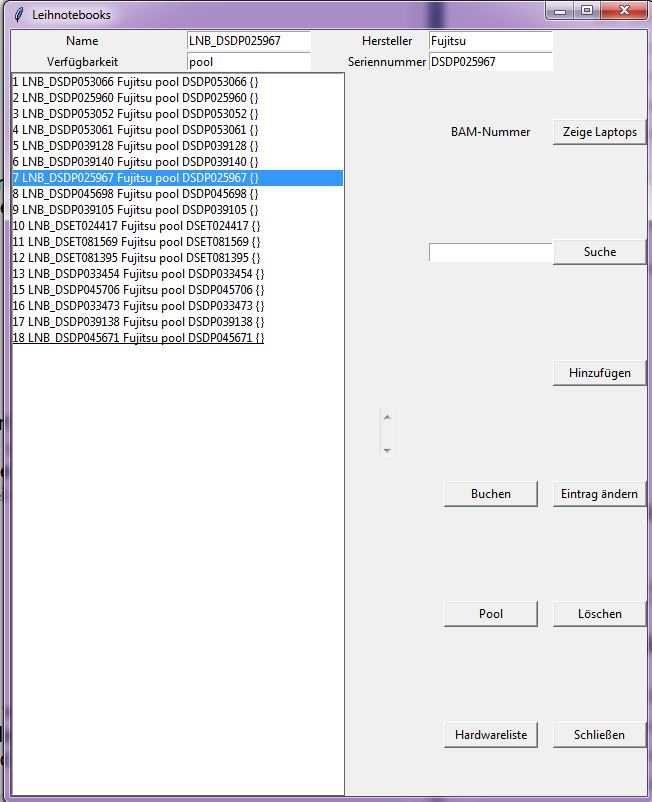
\includegraphics[width=0.7\textwidth]{frontend.jpg}
  \caption{Datenbank-Tool}
  \label{fig:Bild1}
\end{figure}

\noindent
Der Benutzer gibt auf der Ticket-Seite das BAM (Ticketnummer) zu der Bestellung im System auf der Seite an, damit diese einem Auftrag zugeordnet werden kann. Danach wird die Anzahl an benötigten Laptops eingegeben und ob es sich um das Service- oder das Banknetz handelt. Durch den Input auf dem Server werden die Funktionen des Datenbank-Tools aufgerufen und die frei verfügbaren Laptops automatisch in der Datenbank zu buchen und entsprechend auf dem Übergabeprotokoll zu vermerken. Daraufhin wird automatisch eine E-Mail mit dem entsprechenden Lieferschein, welcher die benötigte Hardware auflistet, an meine E-Mail geschickt. Die Anzahl der jeweiligen Hardwarekomponenten wird anhand von bestehenden Konventionen automatisch vom Programm erstellt und berechnet. So wurden zum Beispiel für jeweils fünf Laptops immer ein Switch verschickt. Diese Funktionalitäten wurden in attach.py implementiert, welche in die app.py importiert und von dort aufgerufen werden. 
\begin{figure}[H] 
  \centering
     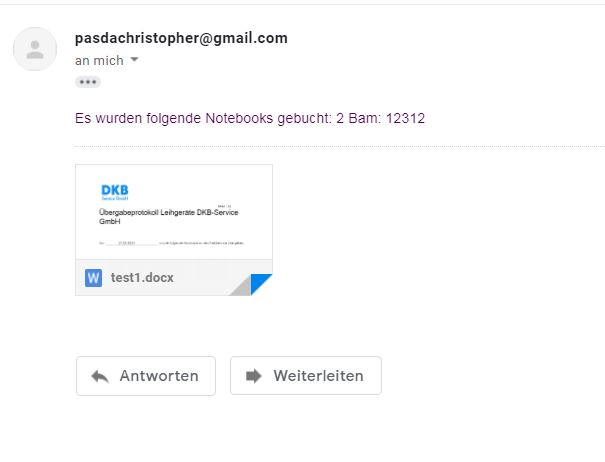
\includegraphics[width=1\textwidth]{email.jpg}
  \caption{Übergabeprotokoll}
  \label{fig:Bild1}
\end{figure}

\noindent
Um das Schicken der E-Mail und ihres Anhangs zu ermöglichen, wurde die smtplib verwendet. Bevor die E-Mail verschickt wird, wird aus der app.py über das Frontend das Übergabeprotokoll erstellt. Dazu wurden mittels der Bibliothek mailmerge Platzhalter in einem Template-Übergabeprotokoll erstellt, welche dann individuell geändert werden können. Diese werden dann mit den Daten aus der Datenbank fusioniert, umbenannt und per E-Mail verschickt.
\\

\noindent
\textbf{Fazit:}
\\ 

\noindent
In diesem Projekt konnte ich mich viel mit Python beschäftigen. Dabei wurden die Grundkenntnisse über Vektoren, For-Schleifen, Input-handling und der Umgang mit Bibliotheken vorausgesetzt. Besonders hängengeblieben sind dabei die GUI-Programmierung und der Umgang mit Datenbanken, welchen ich dank des Moduls an der HTW noch vertiefen konnte. Ich profitierte zudem von den vielen praktischen Projekten, zum Beispiel in Software Engineering, in denen ich meist Python verwendet. So konnte ich schon dort erste Erfahrungen in der Programmierung einer Benutzeroberfläche sammeln, was mir in diesem Projekt sehr zu Gute kam. Ich möchte hier erwähnen, dass sich die vielen praktischen Projekte an der HTW wirklich sehr positiv auf die Arbeit bei der DKB auswirkten und ich entsprechend froh bin, dass der Studiengang Computer Engineering so viel Praxisrelevanz zu bieten hatte. Der Code befindete sich auf dem Git-Repository.

\subsection{Projekt Serien- und Imeinummer zu Excel}
\label{Projekt Serien- und Imeinummer zu Excell}

Nach dem ersten Projekt analysierte ich Abläufe und befragte Kollegen bei welchen Prozessen ihrer Meinung nach viel Zeit verloren geht und welche deshalb optimiert werden könnten. So fand ich heraus, dass neu-gelieferte Hardware händisch eingescannt und in einer Excel-Tabelle registriert werden muss. An den Verpackungen von iPhones, iPads und Laptops befanden sich außen Barcodes (repräsentativ für die jeweilige Serial- und Imei-Nummer der Hardware), welche mittels eines Scanners eingescannt und in einer Excel-Tabelle festgehalten wurden. Diese Excel-Tabelle musste danach an Beschaffung geschickt werden, sodass diese die iPads in die Datenbank einpflegen konnten. Dieser Prozess war sehr aufwändig und zeitraubend, da die Barcodes sehr klein und schwer genau zu Treffen waren. So entschied ich mich zu versuchen mit Python und der Bibliothek Tesseract eine Bilderkennung zu programmieren, welche die Barcodes anhand eines Bildes in einer Excel-Tabelle speichern konnte, sodass lediglich ein Foto von den Barcodes eines jeden Kartons gemacht werden musste. Idealerweise sollte der erstellte Excel-Tabelle direkt an Beschaffung geschickt werden.
\begin{figure}[H] 
  \centering
     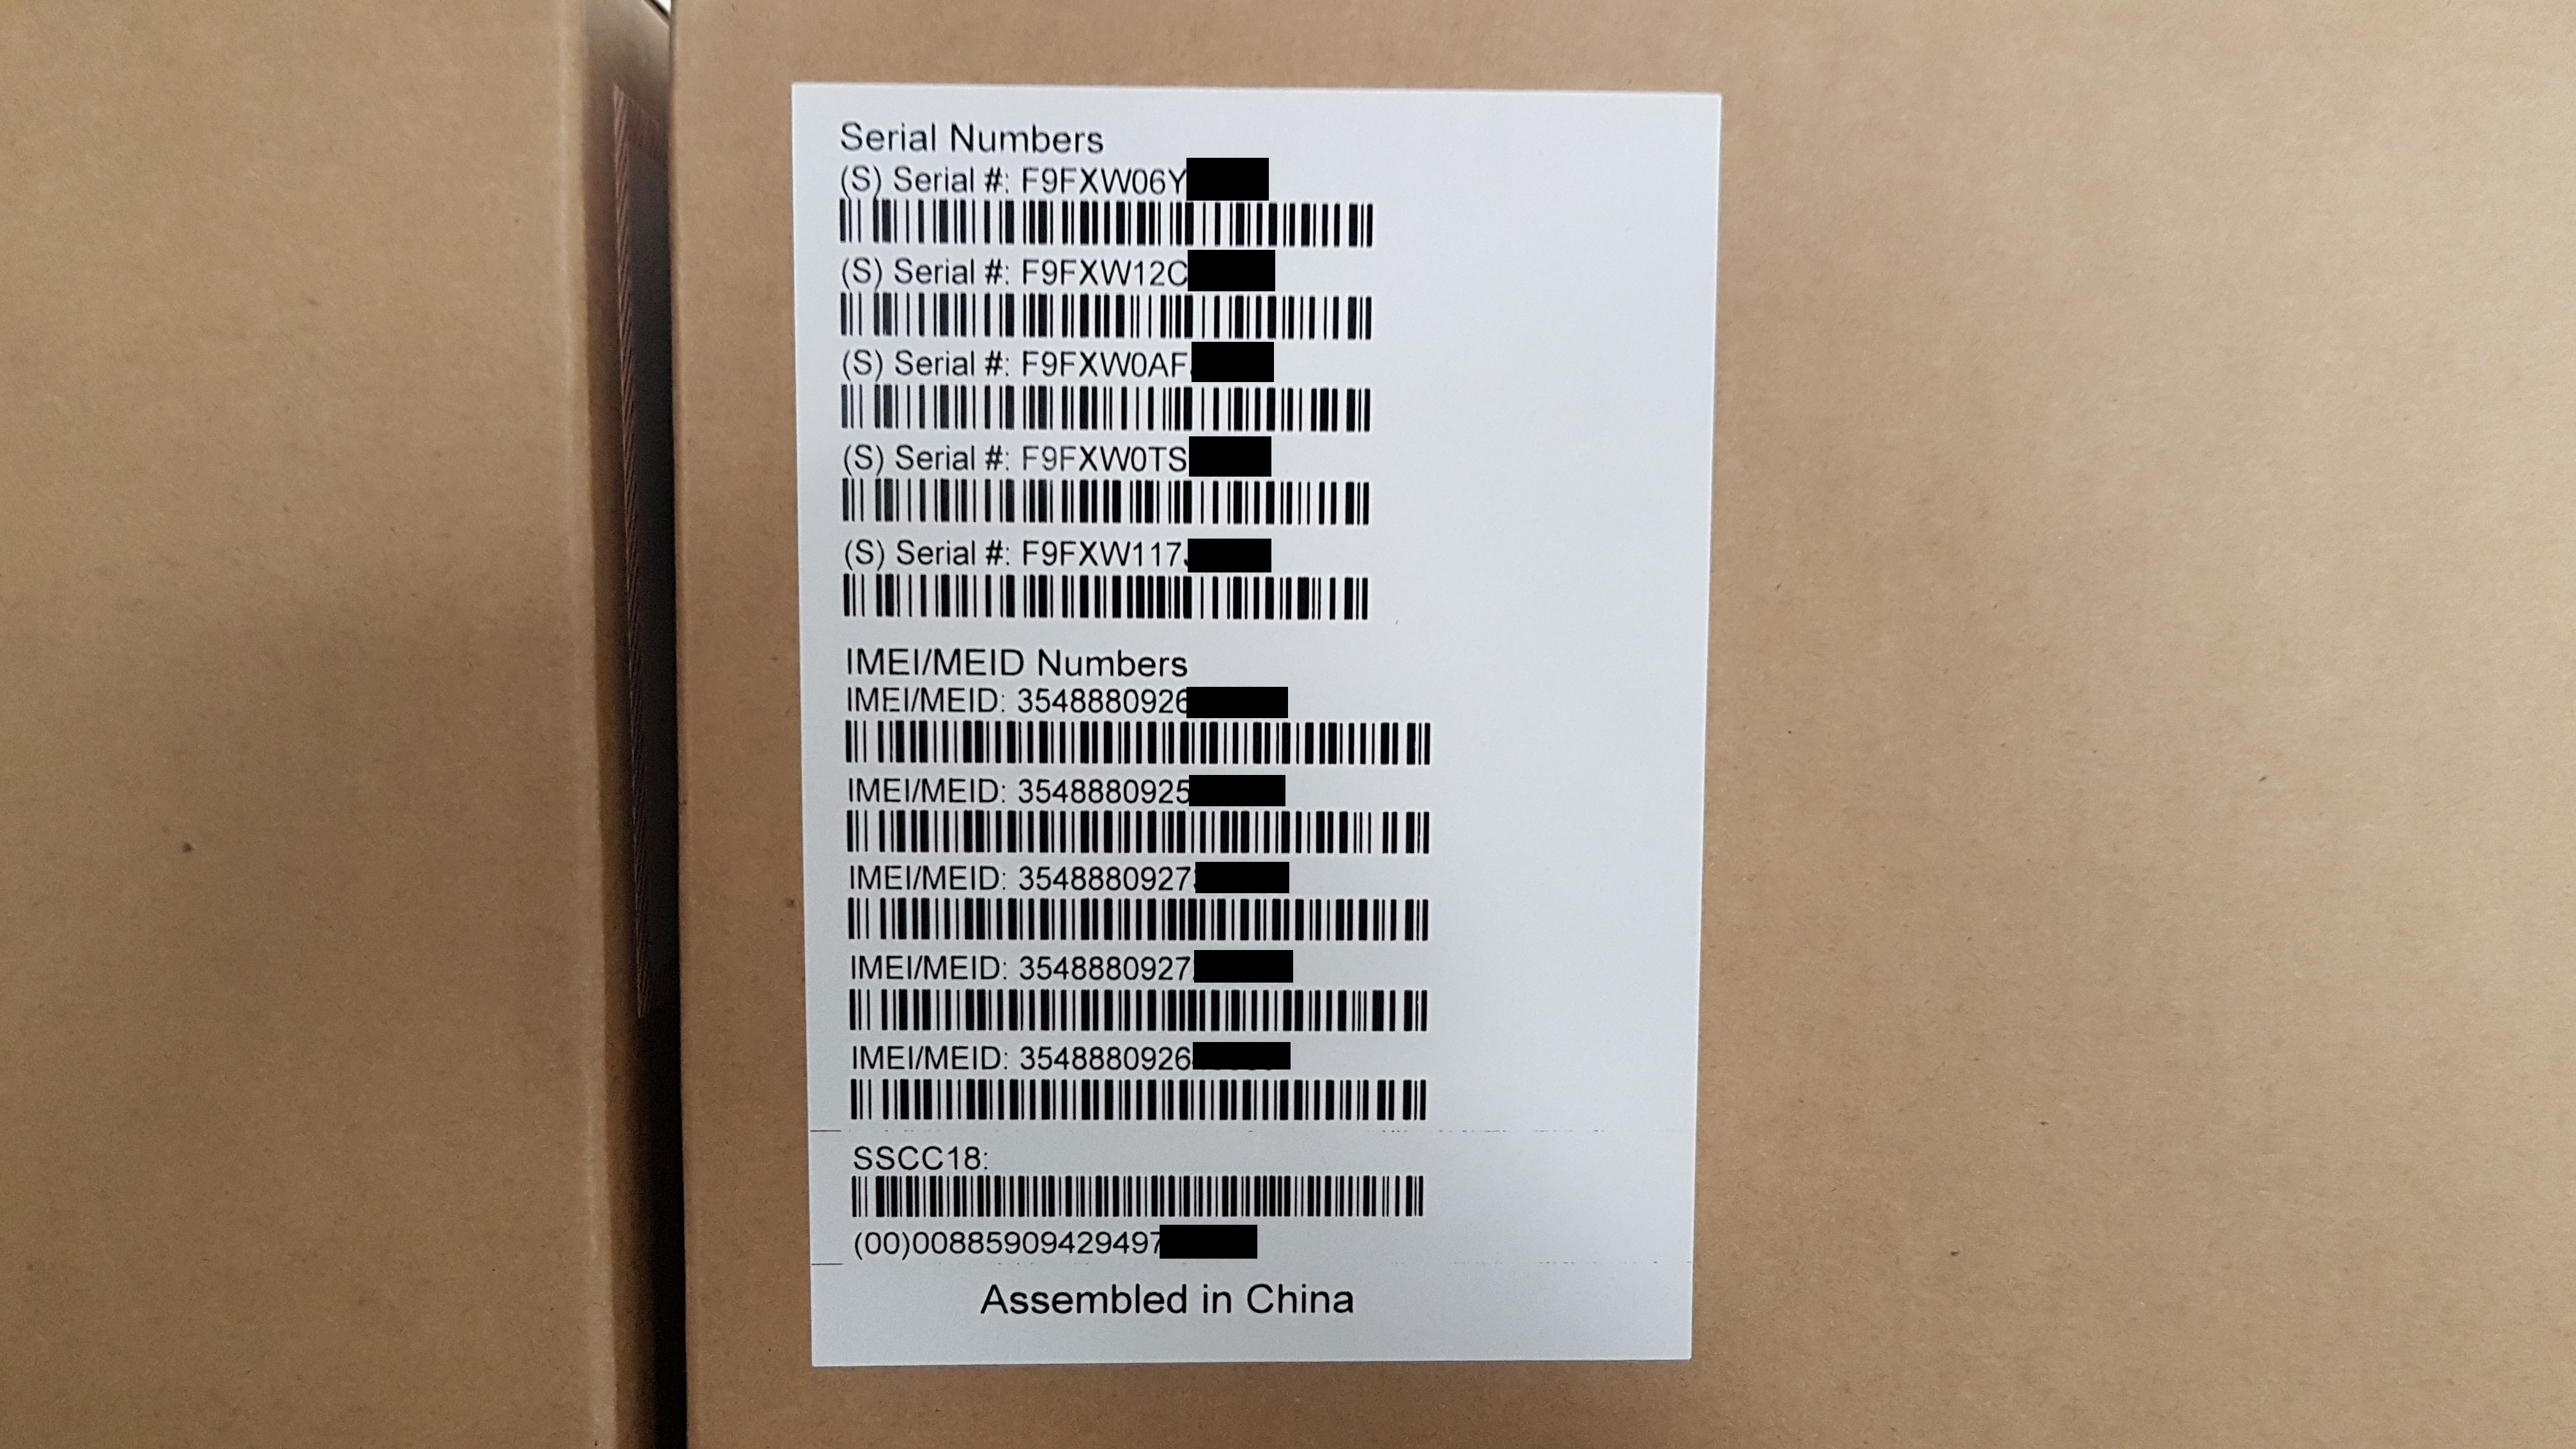
\includegraphics[width=1\textwidth]{etikett.jpg}
  \caption{Etikett iPads (zensiert aus Datenschutz)}
  \label{fig:Bild1}
\end{figure}
\noindent 
Um dies umzusetzen experimentierte ich in den ersten Wochen viel mit der Bilderkennung und der Vorverarbeitung, damit vernünftige Resultate erzielt werden konnten. Besonders wichtig bei der Texterkennung waren das Umwandeln in ein Grauwertbild, das Skallieren und Filtern des Bildes. Das Ziel dabei ist die Kanten der Ziffern zu schärfen, um so durch den Algorithmus bessere Ergebnisse zu erzielen. 
\begin{figure}[H] 
  \centering
     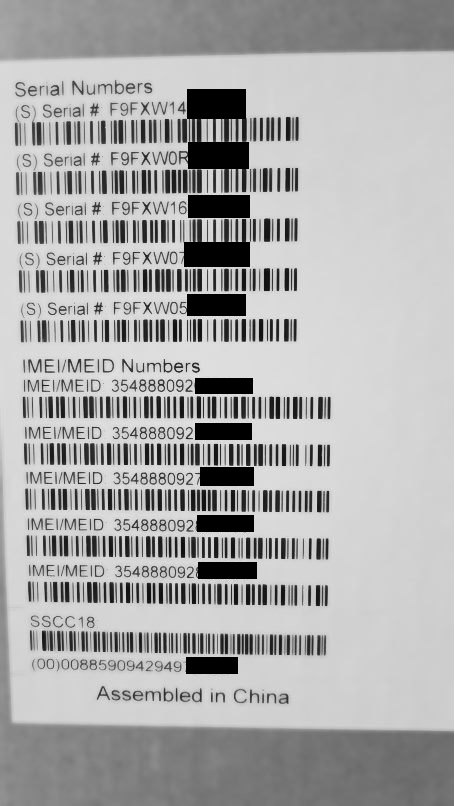
\includegraphics[width=0.4\textwidth]{serial.png}
  \caption{Vorverarbeitetes Bild}
  \label{fig:Bild1}
\end{figure}
\noindent
Dieses Bild wird der Funktion von Tesseract übergeben und daraus werden die Buchstaben mittels Algorithmus in einen String umgewandelt. Dieser String wird danach per Regex nach der Serien- und Imeinummer gefiltert und diese in einer Excel-Liste als Tupel gespeichert.
\begin{figure}[H] 
  \centering
     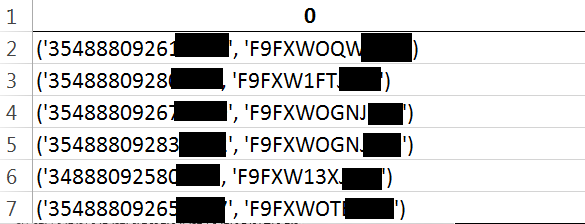
\includegraphics[width=1\textwidth]{tupel.png}
  \caption{Ergebnis als Excel-Liste}
  \label{fig:Bild1}
\end{figure}
\noindent
Aufgerufen werden die Funktion von der Hauptdatei serial.py. In diesem Script befindet sich eine While-Schleife, welche den Userinput verwaltet und die Funktionen von image.py aufruft. 
Es stellte sich heraus, dass es doch sehr schwer war ein verlässliches Ergebnis zu erzielen, bei dem wirklich jede Serien- und Imeinummer korrekt erkannt und in der Excel-Tabelle gespeichert werden konnte. Da dieser Prozess eine einhundertprozentige Zuverlässigkeit gewährleisten musste, schaffte es das Script trotz ca. 95\%iger Erkennungsrate nicht eingesetzt zu werden, da es immer wieder vorkam, dass eine Imei- oder Seriennummer nicht korrekt erkannt wurde. 
\\

\noindent
\textbf{Fazit:}
\\ 

\noindent
Während diesem Projekte lernte ich, dass es ungemein wichtig ist, dass der geschriebene Code verlässlich ist und dass man die Verantwortung trägt, wenn dabei Probleme auftreten und dass es auch sein kann, dass ein Projekt nicht im ersten Anlauf gelingt. Des weiteren verbesserte sich mein Umgang mit Python und der automatischen Bilderkennung. Der Code zu dem Script befindet sich auf dem Git. 





